\section{Hardware}

\subsection{Accellerometer}

\begin{figure}[h]
	\hfill\begin{minipage}{.3\textwidth}\centering
		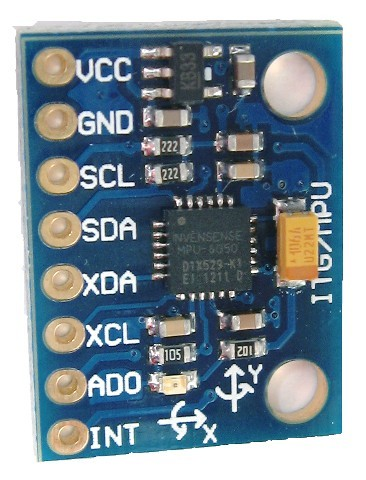
\includegraphics[scale=0.2]{Billeder/mpu-6050.jpg}
		\caption{MPU-6050\\Breakout Board}
		\label{fig:MPU-6050-Breakout}
	\end{minipage}
\end{figure}

\subsection{Lap sensor}

Til at holde øje med når bilen krydsede målstregen, faldt valget på en CNY70 optisk sensor. Den består af en infrarød lysdiode og en phototransistor bygget ind i samme hus. Dioden sender hele tiden infrarødt lys ud gennem et lille vindue, og hvis der er en flade tæt på til at reflektere lyset, vil det blive opfanget af phototransistoren, der sidder ved siden af dioden bag et lysfilter. Mængden af lys der bliver reflekteret tilbage afhænger af afstanden til fladen og typen af materiale der er på overfladen - en hvidt malet streg vil for eksempel reflektere mere lys tilbage end en sort materet overflade.

For at gøre signalet fra sensoren brugbart for microcontrolleren, ville vi bruge en komparator til at digitalisere outputtet. Oprindeligt var planen at bruge en LM311 comparator, men det viste sig at den interne komparator i microcontrolleren lige så nemt kunne bruges til det formål, og så ville der også skæres ned på antallet af eksterne komponenter og derved mindske pladsforbruget på vores print. En anden fordel ved at bruge den interne komparator, er at det bliver muligt at bruge den interne spændingsreference på 2.56 V som input til komparatoren. Så er det bare et spørgsmål om at dimensionere outputtet fra CNY70 sensoren med en modstand, så spændingen der kommer fra den sorte overflade på banen ligger under 2.56V og spændingen fra den hvide målstreg ligger over. Microcontrolleren aflæser komparatoren ved at se på outputtet fra den, og det kan sættes op så den sender et interrupt, når der kommer en rising eller falling edge eller når outputtet skifter tilstand. Med denne løsning bruges der kun tre eksterne komponenter - en modstand hver til henholdsvis lysdioden og phototransistoren samt CNY70 sensoren. Modstanden til lysdioden blev sat til 150 ohm, så der løber godt 30 mA i det kredsløb. For at opfylde spændingskravene til komparatoren blev der brugt en 22 kilo-ohms modstand - det gav en spænding på banen omkring 0.8 V og en spænding på målstregen på ca 4.5 V.

\subsection{Tachometer}

Til at måle omdrejningshastigheden på bilen, samt at opfylde kravet om en elektrofysisk sensor/aktuator, blev der valgt en analog hall sensor som monteredes på motoren. Sensoren har tre ben - et til 5 V, et til stel og et output. Outputtet ligger og svinger omkring 2.5 V og ændrer sig i positiv eller negativ retning alt afhængigt af, hvordan den magnetiske flux ændrer sig i nærheden af sensoren. Når motoren kører vil man på hall sensorens output så kunne måle, når polerne passerer tæt forbi sensoren. Det giver til gengæld et svagt og noget støjet signal, der skal behandles for at microcontrolleren kan bruge det til noget. Det rå signal havde en peak-to-peak spænding på 100-200 mV, så det var ret vigtigt først at få det forstærket op. Det havde også den tilføjede bonus at skære noget af den mere højfrekvente støj fra, fordi den forstærker vi valgte, en instrumenteringsforstærker AD623, havde en knækfrekvens på godt og vel 90 kHz under de forhold vi arbejdede under. 

\begin{figure}[h]

	\centering
		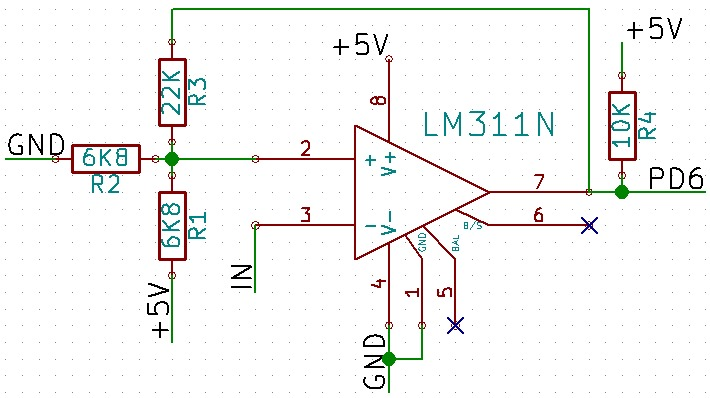
\includegraphics[scale=0.3]{Billeder/Schmitt.jpg}
	\caption{Diagram over schmitt trigger kredsløbet.}
	\label{fig:Schmitt}
	
\end{figure}

Ud fra de første målinger, viste det sig at den lave del af signalet var meget støjfyldt og svær at behandle, så vi valgte at skære den del af signalet fra med et offset på forstærkeren se figur \ref{fig:Signal1}. Offsettet blev styret af et potentiometer, der blev brugt som en slags justerbar referencespænding.

\begin{figure}[h]

	\centering
		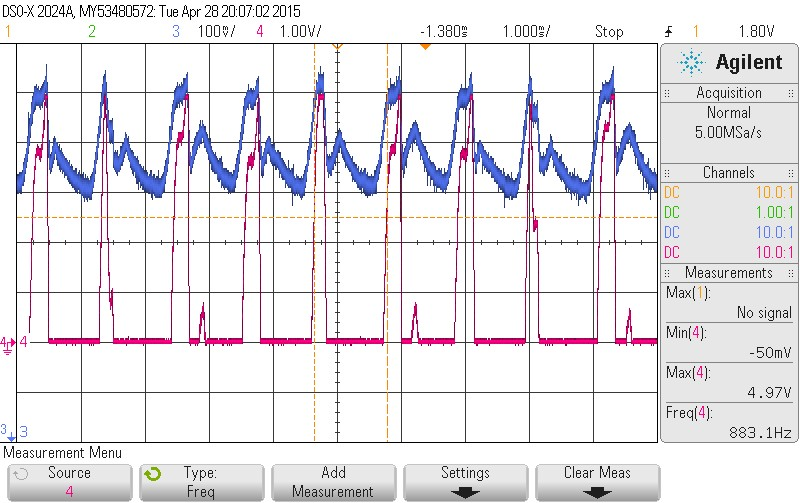
\includegraphics[scale=0.4]{Billeder/Signal1.jpg}
	\caption{Her ses signalet fra hall sensoren før (blå) og efter (lyserød) det er blevet behandlet af forstærkeren.}
	\label{fig:Signal1}
	
\end{figure}

For at digitalisere signalet, så microcontrolleren kunne behandle det, blev der brugt en komparator igen - denne gang som en schmitt trigger for at formindske fejl. Det var ikke nødvendigt at designe spændingstærsklerne på schmitt triggeren så præcist. De skulle bare ligge relativt langt fra hinanden, så eventuel støj ikke kunne få den til at skifte tilstand utilsigtet. Ud fra  målinger med oscilloskop viste det sig, at et spænd på over 0.5 V var rigeligt til at forhindre støj i at få schmitt triggeren til at skifte tilstand.

\begin{equation}
V_{TL} = \dfrac{R_{2}*R_{3}}{R_{2}*R_{3}+R_{1}(R_{2}+R_{3})}*5V
\label{eq:Vtl}
\end{equation}


\begin{equation}
V_{TH} = \left(\dfrac{R_{1}*R_{2}}{R_{1}*R_{2}+(R_{1}+R_{2})(R_{3}+R_{4})} + \dfrac{R_{2}(R_{3}+R_{4})}{R_{2}(R_{3}+R_{4})+R_{1}(R_{2}+R_{3}+R_{4})}\right)*5V
\label{eq:Vth}
\end{equation}



Modstandsværdierne blev dikteret af udvalget på komponentlageret, og ved hjælp af ligning \eqref{eq:Vtl} og \eqref{eq:Vth} designede vi spændingstærskler på henholdsvis 2.2 V og 2.8 V. 

\subsection{Bremse}

\subsection{Elektromagnet}